% flashcards-title: Kilometer and meter conversion map
% flashcards-desc: Two horizontal lines with zeros aligned at the left. The upper line has labeled marks at zero, one, two, and three kilometers; the lower line has labeled marks at zero, one thousand, two thousand, and three thousand meters. Dashed vertical guides join each kilometer mark to the meter mark directly below it, and a dot on the upper line between the two and three kilometer marks has a dashed guide leading down to a question mark on the lower line.
\documentclass[tikz]{standalone}
\usetikzlibrary{arrows.meta,patterns}

\definecolor{qraNavy}{HTML}{17324D}
\definecolor{qraBlue}{HTML}{2B6CB0}
\definecolor{qraGold}{HTML}{B7791F}
\definecolor{qraPale}{HTML}{EAF2F8}
\definecolor{qraGray}{HTML}{5C6773}

\tikzset{
  qra axis/.style={draw=qraNavy, line width=1.2pt},
  qra tick/.style={draw=qraNavy, line width=1pt},
  qra guide/.style={draw=qraGray, densely dashed, line width=0.8pt},
  qra counter/.style={circle, draw=qraNavy, fill=qraPale, line width=0.9pt, minimum size=7mm, inner sep=0pt},
  qra label/.style={font=\sffamily\bfseries, text=qraNavy},
  qra small label/.style={font=\sffamily, text=qraNavy},
}

\begin{document}
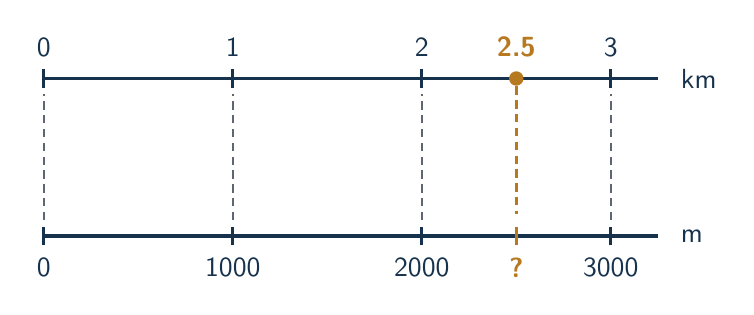
\begin{tikzpicture}[x=2.4cm,y=1cm]
  % pairing guides between matching marks
  \foreach \x in {0,1,2,3}
    \draw[qra guide] (\x,0.2) -- (\x,1.8);
  % highlighted guide for the queried value
  \draw[qra guide, draw=qraGold, line width=1pt] (2.5,1.9) -- (2.5,0.28);
  % top line: kilometers
  \draw[qra axis] (0,2) -- (3.25,2);
  \foreach \x in {0,1,2,3} {
    \draw[qra tick] (\x,1.88) -- (\x,2.12);
    \node[qra small label, above] at (\x,2.16) {\x};
  }
  \node[qra small label, anchor=west] at (3.32,2) {km};
  \fill[qraGold] (2.5,2) circle [radius=2.6pt];
  \node[qra label, above, text=qraGold] at (2.5,2.16) {2.5};
  % bottom line: meters
  \draw[qra axis] (0,0) -- (3.25,0);
  \foreach \x/\l in {0/0,1/1000,2/2000,3/3000} {
    \draw[qra tick] (\x,-0.12) -- (\x,0.12);
    \node[qra small label, below] at (\x,-0.16) {\l};
  }
  \node[qra small label, anchor=west] at (3.32,0) {m};
  \draw[qra tick, draw=qraGold] (2.5,-0.12) -- (2.5,0.12);
  \node[qra label, below, text=qraGold] at (2.5,-0.16) {?};
\end{tikzpicture}
\end{document}
